\documentclass[conference]{IEEEtran}
\IEEEoverridecommandlockouts
% The preceding line is only needed to identify funding in the first footnote. If that is unneeded, please comment it out.
\usepackage{cite}
\usepackage{amsmath,amssymb,amsfonts}
\usepackage{algorithmic}
\usepackage{graphicx}
\usepackage{textcomp}
\usepackage{xcolor}
\usepackage{authblk}
\usepackage{amsthm}
\newtheorem{lem}{Lemma}
\def\BibTeX{{\rm B\kern-.05em{\sc i\kern-.025em b}\kern-.08em
    T\kern-.1667em\lower.7ex\hbox{E}\kern-.125emX}}
\begin{document}

\title{Analytical Optimal Solution of Selfish Node Detection with $2$-hop Constraints in OppNets: A Pontryagin's Maximum Principle Approach
}
\author[1,2,3]{Yang Gao}
\author[1,2,3]{Jun Tao}
\author[1,2]{Zuyan Wang}
\author[1,3]{Wenqiang Li}

\affil[1]{School of Cyber Sci. \& Engr., Southeast University, Nanjing, China}
\affil[2]{Key Lab of CNII, MOE, Southeast University, Nanjing, China}
\affil[3]{Jiangsu Provincial Key Laboratory of Computer Network Technology, Southeast University, Nanjing, China \protect\\
Email: \{yanggao, juntao, zuyan94, wqli\}@seu.edu.cn}

%\author{\IEEEauthorblockN{Yang Gao}
%\IEEEauthorblockA{\textit{Southeast University} \\
%Nanjing, China \\
%yanggao@seu.edu.cn}
%\and
%\IEEEauthorblockN{Jun Tao\thanks{Corresponding author: Jun Tao.}}
%\IEEEauthorblockA{\textit{Southeast University} \\
%Nanjing, China \\
%juntao@seu.edu.cn}
%\and
%\IEEEauthorblockN{Zuyan Wang}
%\IEEEauthorblockA{\textit{Southeast University} \\
%Nanjing, China \\
%zuyan94@seu.edu.cn}
%\and
%\IEEEauthorblockN{Wenqiang Li}
%\IEEEauthorblockA{\textit{Southeast University} \\
%Nanjing, China \\
%wqli@seu.edu.cn}
%}

\maketitle

\begin{abstract}
Selfish node detection offers an effective means
to mitigate the routing performance degradation
caused by selfish behaviors in Opportunistic Networks (OppNets),
but leads to the extra network overload and computation cost.
%due to the detection behaviors.
Most existing effort in the literature focuses on 
exploring the detection methods
based on the traffic analysis or the cooperations among nodes.
%However, the detection brings about
%the detection cost, e.g. energy, bandwidth, revenue,
%as well as the decrement of selfish nodes.
In this paper, we investigate the state transition of nodes
in the message dissemination without detection.
Specifically, the Ordinary Differential Equation (ODE) is constructed 
to approximatively model the periodic detection
with complete detection requirement.
Then we propose the optimal detection solution
with the Pontryagin's maximum principle, 
and mathematically deduce the right detection time 
%the moment of triggering detection on/off
during the message lifetime.
The model soundness is verified statistically
and the analysis accuracy is evaluated via extensive simulations.
The experiments also show that our solution can
achieve the tradeoff between the reward and the detection cost.
%reduce the combinational cost of the wasted reward and the detection.
%based on RWP trace and Shanghai taxi trace.
%Extensive simulations show that
%our scheme outperforms
%the benchmarks, including SDBG, Li and MDS,
%in terms of the delivery ratio in various scenarios.
\end{abstract}


\begin{IEEEkeywords}
Selfish Node Detection, Ordinary Differential Equation,
Pontryagin's maximal principle
\end{IEEEkeywords}

\section{Introduction}
\label{sec:intro}
Exploiting mobile nodes to transmit message in
opportunistic networks(OppNets) has been attracting
increasing research attentions
\cite{DBLP:conf/sigcomm/SouzaMSMCC16,
DBLP:conf/infocom/LuSP16,
DBLP:conf/mobicom/RadenkovicH17,
DBLP:conf/infocom/SakaiSK19,
DBLP:journals/comsur/JedariXN18,
DBLP:journals/tmc/LoretiB20}.
With a widespread use and availability of
mobile communication devices, numerous applications
emerge based on message transmission in OppNets, especially 
in mobile social networks (OMSNs).
Opportunistic computing utilize the shared resources
in  OMSNs to provide a platform for the execution of
distributed computing tasks,

The main contributions are as follows:

\begin{itemize}
\item {we formulate the ordinary differential equation model (ODE)
to capture and analytically evaluate the state transition of nodes
in OppNets without detection and with complete detection.}
\item {we propose an optimal solution of selfish node detection
based on the Pontryagin's maximum principle
to achieve the tradeoff between the detection cost
and the reward of selfish behaviors.}
\item {we conduct experiments to evaluate
the effectiveness of the proposed model
and the optimal selfish detection solution 
in terms of the total cost, the wasted reward and the node state transition.}
\end{itemize}

The rest of this paper is organized as follows.
The literature is reviewed in Section~\ref{sec:related}.
We formulate the problem in Section~\ref{sec:preli}.
The change of network state without detection and with fully detection
is investigated in Section~\ref{sec:ode_model}.
The optimal solution of the selfish detection in OppNets
is presented in Section~\ref{sec:opt_detect},
and evaluated in Section~\ref{sec:pe}.
The paper concludes in Section~\ref{sec:conclude}.

\section{Related Work}
\label{sec:related}
OppNets, which face two challenges,
i.e., energy efficiency and network management cost,
are expected to accommodate participants
with low-delay and cost-effective services.
Therefore, many research works targeted to address these issues.

\subsection{Message Relaying in OppNets}
The primary goal of message forwarding in OppNets
is to exploit the nodes' contact, context,
and social information to improve
the message delivery performance
in terms of different metrics (e.g.,
delivery ratio, delay, overhead,
energy consumption and privacy).
Geo-casting routing protocols, like 
LoSeRo~\cite{DBLP:journals/tmc/CostantinoMMS20},
exploited knowledge of the most frequently visited
to route message in OppNets
and achieved a significant high delivery rate.
Then onion-based anonymous routing
approach~\cite{DBLP:conf/icdcs/SakaiSKWA16}
and ePRIVO~\cite{DBLP:journals/tvt/MagaiaBPC18} were 
proposed to keep users' information private.
To achieve the tradeoff between the delivery ratio
and forwarding cost,
game theory was introduced to
optimize the network configuration in MANETs
for more efficient energy-aware routing
in~\cite{DBLP:journals/monet/MaoZ15}.
%For MOSNs, which exhibits 
Based on a Nested Core-Periphery Hierarchy (NCPH),
\cite{DBLP:journals/tvt/Zheng017} presented
an up-and-down routing protocol,
which can achieve the proper balance
among the data delivery delay, ratio, and cost.
\cite{DBLP:journals/adhoc/RosasGH20} proposed
a context-aware self-adaptive routing protocol
that is able to adapt to different scenarios.

The majority of aforementioned protocols
assume that mobile nodes are willing 
to participate in data delivery.
Nevertheless,
rational nodes in OppNets have strategic interactions
and may exhibit selfish behaviors.
In order to mitigate the performance degradation
caused by the selfishness,
much effort has been made to explore
appropriate incentive mechanisms
to encourage selfish nodes to
participate in data relaying.
For example, the tit-for-tat (TFT)-based scheme,
which forces nodes to exchange the same number
of messages during an opportunistic contact,
was introduced to ensure that 
mobile nodes provide better forwarding services 
for cooperative nodes,
and protect the network against the harm of selfish behaviors
in~\cite{DBLP:journals/tmc/MastronardePXLS16,
DBLP:journals/twc/HsuD17}.
Trust and reputation-based
schemes were adopted to build direct trust relationships
or indirect trust recommendations 
among mobile
nodes~\cite{DBLP:journals/tvt/ChenLWW16,DBLP:conf/mdm/JethawaM18}.
Eventually, better services were provided
for nodes with high reputation
or strong trust relationships.
Credit-based schemes, such as SEIR~\cite{DBLP:conf/ciss/ChhabraVS17},
Multicent~\cite{DBLP:journals/tpds/ChenSY15},
were designed to encourage the node participation
in data relaying 
by rewarding the cooperative nodes
and punishing the selfish nodes.
%via various virtual credits.
%by employing various forms
%of the virtual credit to

\subsection{Abnormal Behavior Detections in OppNets}
\begin{figure}
  \centering
  {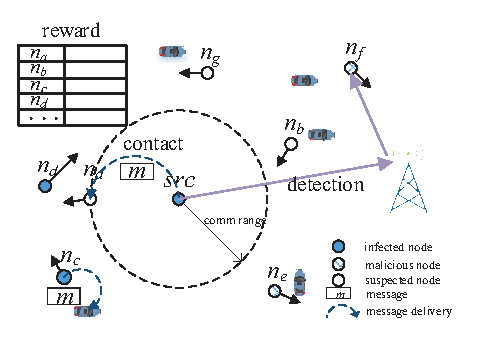
\includegraphics[width=0.47\textwidth]{fig/sketch.eps}}
     \caption{Reward and detection of the selfish nodes in OppNets.}
     \label{fig:sketch}
\end{figure}
Due to the openness of
the wireless communication and the limitations of the
`store-carry-forward' paradigm,
the performance of data delivery in OppNets may be reduced
by abnormal behaviors.
For example,
the selfish behaviors will seriously degrade
the efficiency of data offloading
and the malicious behaviors
will disrupt the normal communications 
between the nodes and the network
throughput deeply~\cite{DBLP:journals/comsur/JedariXN18}.
It is critical to
identify the abnormal node behaviors from network accurately 
and promote the participation of nodes
in the data relaying and the resource sharing.

Observing the importance of selfish behavior detection
schemes for the OppNets,
%the research attentions were attracted in
%a lot of efforts were
a lot of works were
put into its design~\cite{DBLP:journals/fgcs/JedariXCDTA19, Zhou2015Incentive, Chen2014Dynamic, DBLP:journals/tdsc/ChoC18, Wang2016A}.
In~\cite{DBLP:journals/fgcs/JedariXCDTA19},
a general altruism model,
called SoWatch,
was utilized to
distinguish individually selfish behavior 
and socially selfish behavior.
It also showed that the individual 
and social preferences of selfish nodes
may mitigate the cooperation in data relaying.
An incentive-driven and freshness-aware 
pub/sub content dissemination scheme
was proposed in~\cite{Zhou2015Incentive},
with the objective of 
maximizing the utility of the content inventory 
stored in node's buffer.
\cite{Chen2014Dynamic} proposed a dynamic trust management protocol,
in which `healthiness' and
`unselfishness' are considered as two social trust metrics.
A more comprehensive set of performance metrics to characterize QoS (Quality of Service)
in the OppNets
was investigated in~\cite{DBLP:journals/tdsc/ChoC18}.
To guaranty the security requirements of the OppNets,
a credit-based
rewarding scheme was proposed in~\cite{Wang2016A}.

On the other hand,
the protection and defense mechanisms for malicious behaviors have
been demanded by the OppNets.
To deal with the blackhole and greyhole attacks
in DTNs,
\cite{Pham2016Detecting} proposed 
a statistical-based detection scheme and
demonstrated its high accuracy.
A secured routing algorithm for the DTNs
was proposed in~\cite{Saha2018Design},
where the information list of malicious nodes 
was delivered by the trusted nodes.
The types and effectiveness of Sybil attacks in OppNets
was introduced by~\cite{Sacha2016Stalk},
with the consideration of various resource and
attack boosting graph faking attempts.
The problem of confidence crisis caused by malicious nodes
was proposed in~\cite{Yao2016Secure},
and a dynamic trust management model
was presented there to solve the problem.
In~\cite{Chen2016Trust},
an adaptive trust management
protocol for social IoTs (Internet of Things) systems was proposed
to choose the trust parameter settings and change node's social conditions.
%Optimization schemes of OppNets can be classified into
%several types, the most typical one tries to formulate
%the transmitting process in terms of a trade-off between
%the network management cost and the transmission performance.
%For example, on optimal neighbor discovery,
%PWEND~\cite{DBLP:journals/adhoc/ChenQLLWYL20} and
%Pharos~\cite{DBLP:conf/secon/Zhu00L19} adopted time model
%for neighbor discovery and investigated the most energy efficient way
%and the least discovery latency, respectively.
%Then for a given energy budget,
%how to optimizing the number of discovered peers was researched
%in~\cite{DBLP:journals/tmc/LoretiB20},
%what is the best achievable discovery latency was addressed
%by~\cite{DBLP:conf/sigcomm/KindtC19}.
%
%As for optimal data forwarding,
%\cite{DBLP:journals/tvt/ZhouLZXF17} proposed an
%efficient time-aware data forwarding strategy(TCCB) for OMNs,
% based on temporal social contact patterns.
% The model performed a close delivery ratio to
% Epidemic but with significantly reduced delivery cost.
%\cite{DBLP:journals/tvt/LiuWXWLY17} introduced
%a centralized heuristic algorithm
%which aimed to discover a tree for multicasting,
%with resource constrained (i.e. the delay-constrained least-const) in MONs.
%Both centralized and decentralized single-copy message forwarding algorithms
%were proposed in~\cite{DBLP:journals/tsipn/ShaghaghianC15},
%which aimed to minimize the expected latencies
%from any node in the Opportunistic DTNs.
%However, aforementioned works just consider one part of
%the message transmission in OppNets,
%\cite{DBLP:journals/tcss/WuDH18} mathematically characterized
%message transmission of the selfish
%and altruistic cases as an optimal control problem,
%whose controlling parameters were chosen according
%to the forwarding rate and beaconing rate, respectively.
%Then the Pontryagin's Maximum Principle was exploited
%to search the problem solution in multiple destinations scenario
%and the optimal control policies were proved to satisfy the threshold form.
%%Wu et al. considered the optimal forwarding and beaconing control problem at the same time in DTN and gave solution based on Pontryagin's Maximum Principle in ~\cite{DBLP:journals/tcss/WuDH18}, where multiple destinations exist.
%
%Minimize the contact duration by optimizing
%mobile data offloading in OMNs is the objective
%of~\cite{DBLP:journals/tits/LiJWZ014,DBLP:conf/icc/WangW18}.
%A mathematical framework to study the problem of
%coding-based mobile data offloading
%was established in~\cite{DBLP:journals/tits/LiJWZ014},
%the authors formulated the problem as a users' interest
%satisfaction maximization problem
%with multiple linear constraints of
%limited storage and efficient scheme
%was proposed to solve it.
%An optimal traffic offloading scheme through
%data partition, which generated forwarding paths
%with possible heterogeneous data chunks,
%was presented in~\cite{DBLP:conf/icc/WangW18}.

%Few these existing works focus on
%optimal control policy, while we introduce it
%for selfish node detection,
%where the scenario is different
%from~\cite{DBLP:journals/tcss/WuDH18} in this paper.
Few existing works focus on
the optimal control policy to balance
the cost of selfish node detection
and the reward to encourage the participation of nodes.
Therefore, we utilize ODEs to model the message dissemination
caused by contacts and detections,
and propose a optimal selfish node detection method
based on the Pontryagin's maximum principle.

\section{Preliminaries}
\label{sec:preli}
% motivation
In the OppNets,
the messages, e.g., advertisements, urgent notifications,
reports and tasks,
always need to be disseminated
to the specific group of users.
As an example, the source node $src$
should disseminate the message $m$,
which will exist from $0$ to $T$,
to the relay nodes,
e.g., vehicles or pedestrians.
There are $N$ relay nodes in the network,
which can replicate, store $m$ and send it further.
Thus the potential coverage area of the message
can be broadened by this network.
To encourage the collaboration of relay nodes,
$src$ should reward the relay node $n_{i}$
$(1 \le i \le N)$ based on the message carrying time,
which means the maximum time-interval
starts from the replication time $\tau_{i}^{s}$
to $T$.
%which starts from the replication time $\tau_{i}^{s}$
%to the message lifetime $T$.
%during which the message are carried by $n_{i}$.
%The message carrying time
%ranges from the replication time ($\tau_{i}$)
%to the message lifetime ($T$).
Since $\tau_{i}^{s}$ is recorded by $src$
at the contact between $src$ and $n_{i}$,
$src$ can calculate the reward
as $\beta (T-\tau_{i}^{s})$, where $\beta$ is the reward per second.
%$n_{i}$ contacts $src$ and replicates $m$.
%Since the message only can be replicated
%from $src$ to the relay node in this paper,
%$src$ can record the replication time $\tau_{i}$.

\begin{figure}
  \centering
  {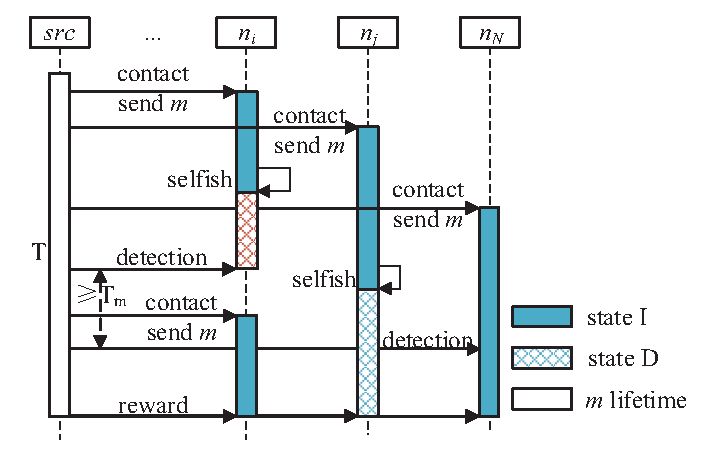
\includegraphics[width=0.47\textwidth]{fig/schedule.eps}}
     \caption{Sate transition of behaviors in time dimension.}
     \label{fig:schedule}
\end{figure}
However, $n_{i}$ may discard $m$
% immediately after the contact
to earn the reward without carrying $m$,
which is the main type of
the selfish behaviors considered in this paper.
To mitigate the behaviors,
$src$ adopts the detection,
%, which is the cost of selfish behaviors.
which can be conducted as follows:
$1$) $src$ selects a detected relay node $n_{r}$
from the $N$ node set randomly;
$2$) $src$ determines the random segment of the message $m_{+}$;
$3$) $src$ sends the query about the checksum of $m_{+}$
to $n_{r}$ via cellular networks 
(or other Internet access technologies);
$4$) If $src$ receives the correct checksum after $T_{m}$,
$n_{r}$ is not a selfish node;
otherwise, $n_{r}$ is a selfish node.
For example, if $n_{i}$ is identified
as a selfish node at time $\tau_{i}^{d}$,
the reward will be computed as $\beta(\tau_{i}^{d} - \tau_{i}^{s})$,
which means that $n_{i}$ will not receive the reward
from $\tau_{i}^{d}$.
The whole process,
including contacts, detections and rewards,
is shown in Fig.~\ref{fig:schedule}.
State $I$ means that the nodes carry $m$.
State $D$ denotes that the nodes have discarded $m$.
Other nodes stay in state $R$.
The contact can make the node,
which is in state $R$ or in state $D$,
transit into state $I$.
The selfish behavior encourages the node to discard the message,
which can still receive the reward from $src$
before being detected.
After the message lifetime,
the reward can be calculated according to
the contacts and the detections recorded in $src$.
In this paper, we propose the optimal random detection strategy
to reduce the detection cost 
caused by the frequent communications through cellular networks
and improve the reward utilization ratio.
%
%to achieve the tradeoff between
%the cost of the random detections and
%the wasted reward of the selfish behaviors.

%1.Poisson process of contacts
%2.Poisson process of being selfish
$E(R(t))$ denotes the expected number of the relay nodes,
which have not contacted $src$ before time $t$.
$E(I(t))$ denotes the expected number of infected relay nodes,
which still carry the message at time $t$.
$E(D(t))$ denotes the expected number of selfish relay nodes,
which have discarded the message 
but are still not found by time $t$.
Similar to \cite{DBLP:journals/tcss/WuDH18} and \cite{CC2007PerfAnaly},
the contacts between any two nodes
can be adequately modeled as Poisson process,
in which the contact rate is $\lambda$.
The total number of relay nodes is $N$,
and $N=R(t)+I(t)+D(t)$, $\forall t \in [0, T]$.
We also assume the rate of a node getting into selfish mode
from state $I$
is the constant parameter $\rho$.
The detection rate $U(t)$,
which means the detections speed at different time,
satisfies $0 \le U(t) \le U_{m}$, $\forall t \in [0, T]$.
For instance, if the minimal detection cycle
$T_{m}$ is that $2$s,
the maximal frequency of detection is
$U_{m} = \frac{1}{T_{m}} = 0.5$ per second.
To simplify the denotations,
we use $R(t)$, $I(t)$ and $D(t)$ to
replace $E(R(t))$, $E(I(t))$ and $E(D(t))$,
respectively.
%Then the main objective of our work is
%to solve the following problem,
The total reward paid to all relay nodes by $src$ is
\begin{equation}
\begin{small}
\label{eq:reward}
\begin{aligned}
P &= \int_{0}^{T} \beta \big( I(t) + D(t) \big)dt,
\end{aligned}
\end{small}
\end{equation}
where $\beta$ is the reward of unit time
paid to a node carrying the message.
$\int_{0}^{T} D(t) dt$ is proportional to the wasted reward.

The optimal random detection problem
in this paper can be formulated as:
\begin{equation}
\begin{small}
\label{eq:obj}
\begin{aligned}
Min: J &= \int_{0}^{T} \big( (1-\alpha) D(t) + \alpha U(t) \big) dt,
\end{aligned}
\end{small}
\end{equation}
which minimizes the linear combination of
the wasted reward and the detection cost through the weight $\alpha$,
$0 < \alpha < 1$.


\section{Message Dissemination Model}
\label{sec:ode_model}
We investigate the selfish detection in this and the following sections.
Specifically, in this section, the ordinary differential equation model
is constructed to capture the state transition and the message dissemination
without detection and with complete detection.
\subsection{Case 1: without detection}
\label{subsec:wo_detc}
\begin{figure}
  \centering
  {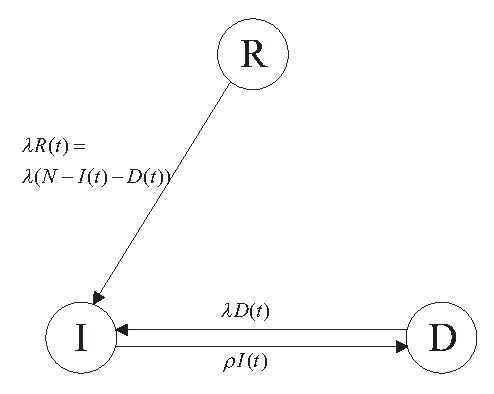
\includegraphics[width=0.23\textwidth]
  {fig/state_transition_no_detect.eps}}
     \caption{State transition of the relay nodes without detection.}
     \label{fig:ss_wo_dt}
\end{figure}
In the case without detection,
the relay node with message can become the selfish node,
but the selfish detection is not conducted by $src$.
Then the state transition is shown
in Fig.~\ref{fig:ss_wo_dt} with the following rules.
The nodes change from state $R$ to state $I$ if they contact $src$.
The corresponding incremental rate of state $I$ is $\lambda R(t)$ at time $t$.
Since the selfish node may also contact $src$ with the contact rate $\lambda$,
the rate of change from state $D$ to state $I$ is $\lambda D(t)$.
Because $N=R(t)+I(t)+D(t)$,
the total incremental rate of $I(t)$ is
$\lambda (R(t)+D(t))=\lambda (N-I(t))$.
Additionally, the rate of change from state $I$ to state $D$ is $\rho I(t)$.
We can obtain the derivative of $I(t)$ with respect to time $t$,
$\frac{\mathrm{d} I(t)}{\mathrm{d} t} = \lambda (N-I(t)) - \rho I(t)$.
Similar to $\frac{\mathrm{d} I(t)}{\mathrm{d} t}$,
we can get the derivative of $D(t)$
and the derivative of $R(t)$ respectively,
i.e., $\frac{\mathrm{d} D(t)}{\mathrm{d} t}$ and
$\frac{\mathrm{d} R(t)}{\mathrm{d} t}$.
Thus the state transition can be represented as
\begin{small}
\begin{equation}
\label{eq:IDR_wo}
\begin{aligned}
\frac{\mathrm{d} I(t)}{\mathrm{d} t} &=  \lambda (N-I(t)) - \rho I(t),\\
\frac{\mathrm{d} D(t)}{\mathrm{d} t} &= - \lambda D(t) + \rho I(t),\\
\frac{\mathrm{d} R(t)}{\mathrm{d} t} &= - \lambda (N-I(t)-D(t)).
\end{aligned}
\end{equation}
\end{small}
Since $I(t)$ in (\ref{eq:IDR_wo}) is formed by the first-order first-power
ordinary differential equations (ODE)~\cite{CC2007PerfAnaly},
we can obtain the general solutions of $I(t)$, that is,
\begin{small}
\begin{equation}
\nonumber
\begin{aligned}
I(t) = C_{I} e^{-(\lambda + \rho)t} + \frac{ \lambda N }{ \lambda + \rho }.
\end{aligned}
\end{equation}
\end{small}
Note that $I(0)=0$, $D(0)=0$ and $R(0)=N$,
which means only $src$ carries the message at time $0$.
Thus $C_{I} = \frac{ -\lambda N }{ \lambda + \rho }$, and
\begin{small}
\begin{equation}
\nonumber
\begin{aligned}
I(t) = \frac{ \lambda N }{ \lambda + \rho }(1- e^{-(\lambda + \rho)t}),
\end{aligned}
\end{equation}
\end{small}
where $0 \le t \le T$.
Similarly, we can calculate the general solution of the first-order ODE $D(t)$
from $\frac{\mathrm{d} D(t)}{\mathrm{d} t} + \lambda D(t) = \rho I(t)$,
\begin{small}
\begin{equation}
\label{eq:D_formula}
\begin{aligned}
D(t) &= C_{D} e^{-\int \lambda dt} + e^{-\int \lambda dt} \int \rho I(t) e^{\int \lambda dt} dt \\
%&= C_{D} e^{- \lambda t} +
%e^{- \lambda t} \int \rho \frac{ \lambda N }{ \lambda + \rho } (1 - e^{-(\lambda + \rho)t}) e^{ \lambda t} dt \\
&= C_{D} e^{- \lambda t} + \frac{ \lambda N }{ \lambda + \rho } e^{-(\lambda + \rho)t} + \frac{ \rho N }{ \lambda + \rho }.
\end{aligned}
\end{equation}
\end{small}
Because of $D(0)=0$,
\begin{small}
\begin{equation}
\nonumber
\begin{aligned}
D(t) &= -N e^{- \lambda t} + \frac{ \lambda N }{ \lambda + \rho } e^{-(\lambda + \rho)t} + \frac{ \rho N }{ \lambda + \rho }.
\end{aligned}
\end{equation}
\end{small}
Since $I(t)+D(t)+R(t)=N$, $0 \le t \le T$,
$R(t)$ can be computed based on the solved solution of $I(t)$ and $D(t)$.
Thus the solution of (\ref{eq:IDR_wo}) can be derived as
\begin{small}
\begin{equation}
\label{eq:IDR_wo_solu}
\begin{aligned}
I(t) &= \frac{ \lambda N }{ \lambda + \rho }(1- e^{-(\lambda + \rho)t}), \\
D(t) &= N (\frac{\lambda e^{-(\lambda + \rho)t} + \rho}{ \lambda + \rho } - e^{- \lambda t}), \\
R(t) &= N e^{- \lambda t},
\end{aligned}
\end{equation}
\end{small}
which depicts the change of the states when the time ranges from $0$ to $T$.
And $I(t)$, $D(t)$, $R(t)$ $\ge 0$ always hold when $t \ge 0$.
From the solutions of $I(t)$, $D(t)$ and $R(t)$,
we can find that $I(t) \rightarrow \frac{ \lambda N }{ \lambda + \rho }$,
$D(t) \rightarrow \frac{ \rho N }{ \lambda + \rho }$
and $R(t) \rightarrow 0$,
when $t \rightarrow + \infty$.
To verify the validity of the ODE model (\ref{eq:IDR_wo}),
we conduct the simulations with randomly settings.
The corresponding results are presented in Section.~\ref{subsec:pe_valid}.

The cost $J$ in (\ref{eq:obj}) also can be calculated based on (\ref{eq:IDR_wo_solu}).
Note that $U(t)=0$, $\forall t$,
in the case without detection.
$J$ is determined by the expected number of selfish nodes $D(t)$,
$0 \le t \le T$,
which is proportional to the reward consumed by selfish behaviors.
Thus $J$ can be computed as
\begin{small}
\begin{equation}
\label{eq:IDR_wo_J}
\begin{aligned}
J &= \int_{0}^{T} (1-\alpha) D(t) dt, \\
&= \int_{0}^{T} (1-\alpha) N (\frac{\lambda e^{-(\lambda + \rho)t} + \rho}{ \lambda + \rho } - e^{- \lambda t}) dt, \\
&= N (1-\alpha) \left( \frac{\lambda (1-e^{-(\lambda+\rho)T})}{ (\lambda + \rho)^{2} }
+ \frac{\rho T}{\lambda + \rho}
- \frac{1-e^{-\lambda T}}{\lambda} \right).
\end{aligned}
\end{equation}
\end{small}
Similarly, we can get the total paid reward in this case
\begin{small}
\begin{equation}
\nonumber
\begin{aligned}
P &= \beta \int_{0}^{T} I(t) + D(t) dt
%&= \beta \int_{0}^{T} (N - N e^{- \lambda t}) dt, \\
= N \beta (T - \frac{ 1 - e^{-\lambda T} }{\lambda} ).
\end{aligned}
\end{equation}
\end{small}
Furthermore, the fraction between the wasted reward and the total paid reward can be obtained as
\begin{small}
\begin{equation}
\nonumber
\begin{aligned}
p = \frac{\int_{0}^{T} D(t) dt}{\int_{0}^{T} I(t) + D(t) dt}
&= \frac{ \frac{\lambda (1-e^{-(\lambda+\rho)T})}{ (\lambda + \rho)^{2} }
+ \frac{\rho T}{\lambda + \rho}
- \frac{1-e^{-\lambda T}}{\lambda} }
{T - \frac{ 1 - e^{-\lambda T} }{\lambda} }.
\end{aligned}
\end{equation}
\end{small}

\subsection{Case 2: with complete detection}
\label{subsec:full_detc}
\begin{figure}
  \centering
  {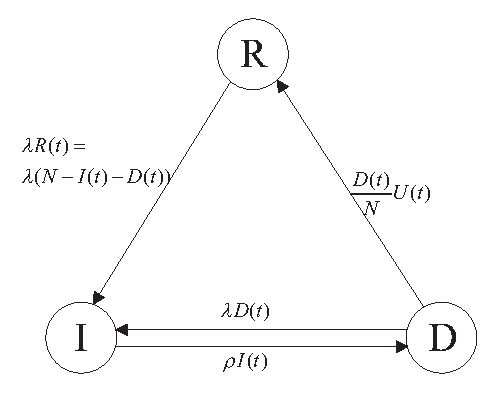
\includegraphics[width=0.23\textwidth]
  {fig/state_transition_detect.eps}}
     \caption{State transition of the relay nodes.}
     \label{fig:ss_dt}
\end{figure}
In the case with complete detection,
$src$ conducts the selfish node detection in the whole message lifetime.
The detections are conducted at
time {$T_{m}$, $2 T_{m}$, $\cdots$, $k T_{m}$},
where $k T_{m} \le T < (k+1) T_{m}$.
In every detection, a randomly selected node $n_{i}$
is checked by $src$ whether $n_{i}$ is a selfish node.
We can find that the decrement of selfish node number
only occurs at the instant $iT_{m}$
in the case with complete detection.

In order to simplify the model,
we exploit a continuous manner to
describe this case with complete detection.
Considering that the checked relay node
is randomly selected from the $N$ node set,
we calculate the probability of selecting a selfish node
as $\frac{D(t)}{N}$.
Since the detection rate is constrained by $U(t)$,
we let $\frac{D(t)}{N}U(t)$ denote
the change rate from state $D$ to state $R$ caused by detections.
Thus the state transition of the fully detection case
is constructed as Fig.~\ref{fig:ss_dt}.
The approximate model of the state transition in the case with complete detection
will be constructed as
\begin{small}
\begin{equation}
\label{eq:IDR_full}
\begin{aligned}
\frac{\mathrm{d} I(t)}{\mathrm{d} t} &=  \lambda (N-I(t)) - \rho I(t),\\
\frac{\mathrm{d} D(t)}{\mathrm{d} t} &= - \lambda D(t) + \rho I(t) - \frac{D(t)}{N} U(t),\\
\frac{\mathrm{d} R(t)}{\mathrm{d} t} &= - \lambda (N-I(t)-D(t)) + \frac{D(t)}{N} U(t),
\end{aligned}
\end{equation}
\end{small}
based on the model in the case without detection (\ref{eq:IDR_wo}).
Here $U(t) = U_{m}$, $\forall t$, $0 \le t \le T$.
The initial state is that $I(0)=D(0)=0$ and $R(0)=N$.
So the solution of $I(t)$, which does not change from $(\ref{eq:IDR_wo_solu})$,
is that $I(t) = \frac{ \lambda N }{ \lambda + \rho }(1- e^{-(\lambda + \rho)t})$.
From $\frac{\mathrm{d} D(t)}{\mathrm{d} t} + (\lambda + \frac{U_{m}}{N}) D(t)= \rho I(t)$,
we can derive that
\begin{small}
\begin{equation}
\nonumber
\begin{aligned}
& D(t) \\
=& C_{2D} e^{\int -(\lambda + \frac{U_{m}}{N}) dt}
+ e^{\int -(\lambda + \frac{U_{m}}{N}) dt} \int \rho I(t) e^{\int (\lambda + \frac{U_{m}}{N}) dt} dt \\
=& C_{2D} e^{-(\lambda + \frac{U_{m}}{N})t}
- \frac{ \rho \lambda N }{ (\lambda + \rho)(\frac{U_{m}}{N} - \rho) } e^{-(\lambda + \rho)t}
+ \frac{ \rho \lambda N }{ (\lambda + \rho)(\lambda + \frac{U_{m}}{N}) }.
\end{aligned}
\end{equation}
\end{small}
Since $D(0) = 0$ and $I(t) + D(t) + R(t) = N$,
%\begin{small}
%\begin{equation}
%\nonumber
%\begin{aligned}
%D(t) =& \frac{ \rho \lambda N }{ \lambda + \rho } \frac{1}{\lambda + \frac{U_{m}}{N}}
%- \frac{\rho \lambda N}{(\lambda + \frac{U_{m}}{N})(\frac{U_{m}}{N} - \rho)}  e^{-(\lambda + \frac{U_{m}}{N})t}\\
%& - \frac{ \rho \lambda N }{ \lambda + \rho } \frac{1}{\frac{U_{m}}{N} - \rho} e^{-(\lambda + \rho)t}
%\end{aligned}
%\end{equation}
%\end{small}
the solution of (\ref{eq:IDR_full}) can be calculated as
\begin{small}
\begin{equation}
\label{eq:IDR_full_solu}
\begin{aligned}
I(t) =& \frac{ \lambda N }{ \lambda + \rho }(1- e^{-(\lambda + \rho)t}),\\
D(t) =& \frac{ \rho \lambda N }{ (\lambda + \rho)(\lambda + \frac{U_{m}}{N}) }
+ \frac{\rho \lambda N}{(\lambda + \frac{U_{m}}{N})(\frac{U_{m}}{N} - \rho)}  e^{-(\lambda + \frac{U_{m}}{N})t}\\
& - \frac{ \rho \lambda N }{ (\lambda + \rho)(\frac{U_{m}}{N} - \rho) } e^{-(\lambda + \rho)t},\\
R(t) =& N - \frac{ \lambda N }{ \lambda + \rho } \left( \frac{\rho}{\lambda + \frac{U_{m}}{N}} + 1 \right)
+ \frac{ \lambda U_{m} }{ (\lambda + \rho)(\frac{U_{m}}{N} - \rho) } e^{-(\lambda + \rho)t}\\
& - \frac{\rho \lambda N}{(\lambda + \frac{U_{m}}{N})(\frac{U_{m}}{N} - \rho)}  e^{-(\lambda + \frac{U_{m}}{N})t}.
\end{aligned}
\end{equation}
\end{small}
We can find that $I(t) \rightarrow \frac{ \lambda N }{ \lambda + \rho }$,
$D(t) \rightarrow \frac{ \rho \lambda N }{ (\lambda + \rho)(\lambda + \frac{U_{m}}{N}) }$,
and $R(t) \rightarrow  N - \frac{ \lambda N }{ \lambda + \rho } \left( \frac{\rho}{\lambda + \frac{U_{m}}{N}} + 1 \right)$
when $t \rightarrow +\infty$ according to (\ref{eq:IDR_full_solu}).
Here $R(+\infty) \neq 0$ in the steady state
is caused by the complete selfish detection.
Based on the approximate model (\ref{eq:IDR_full})
and the corresponding solutions (\ref{eq:IDR_full_solu}),
the estimation of the total cost $\hat{J}$
can be computed as
\begin{small}
\begin{equation}
\label{eq:IDR_full_J}
\begin{aligned}
\hat{J} =& \int_{0}^{T} (1-\alpha) D(t) + \alpha U(t) dt, \\
=& \frac{ (1-\alpha) \rho \lambda N T }{ (\lambda + \rho)(\lambda + \frac{U_{m}}{N}) }
- \frac{(1-\alpha) \rho \lambda N}{ {(\lambda + \frac{U_{m}}{N})}^{2} (\frac{U_{m}}{N} - \rho)}
(e^{-(\lambda + \frac{U_{m}}{N})T} - 1 ) \\
&+ \frac{(1-\alpha) \rho \lambda N }{ {(\lambda + \rho)}^{2} (\frac{U_{m}}{N} - \rho) }
(e^{-(\lambda + \rho)T} - 1 )
+ \alpha T U_{m}.
\end{aligned}
\end{equation}
\end{small}
The reason why (\ref{eq:IDR_full_J}) is the estimation of the cost
is that the decrement of $D(t)$ actually occurs in the end of the detection cycle.
However, the change rate of $D(t)$ in (\ref{eq:IDR_full})
is denoted by $\frac{D(t)}{N}U(t)$ in the above analysis.
So there exists a deviation between the true cost $J$ and the estimated cost $\hat{J}$
in the case with complete detection.
\begin{lem}
When $t \rightarrow +\infty$, $T_{m} \ll T$,
a deviation between $D(t)$ in the approximate model (\ref{eq:IDR_full_solu})
and in the real scenario is limited.
\end{lem}

\begin{proof}
At first we discuss the real scenario of the complete detection case.
Without loss of generality,
assume that $(0, T)$ can be divided into $k$ detection cycles
and a following duration $t_{k+1}$.
Here the $i$-th detection cycle is denoted by $(t_{i-1}, t_{i}]$,
where $t_{i} - t_{i-1} = T_{m}$ and $t_{k+1} < T_{m}$.
In every detection cycle,
$D(t)$ increases from $D(t_{i-1})$ to $D(t_{i}^{-})$
in $(t_{0}, t_{1}^{-})$.
Since the detection occurs at the instant $t_{i}$,
$D(t_{i}^{+}) = \frac{N-1}{N}D(t_{i}^{-})$.
From (\ref{eq:IDR_wo_solu}) we can find that $D(t)$ increases with time in the case
and approaches to the stable state in the case without detection.
In the case with complete detection,
when $t \rightarrow +\infty$,
$D(t)$ also approaches to the stable state,
where $D(t_{i-1}^{+}) = D(t_{i}^{+})$.
We can obtain that
\begin{small}
\begin{equation}
\nonumber
\begin{aligned}
D(t_{i-1}^{+}) = & C_{i} e^{-\lambda t_{i-1}^{+}}
+ \frac{\lambda N}{\lambda + \rho} e^{-(\lambda+\rho)t_{i-1}^{+}}
+ \frac{\rho N}{\lambda+\rho}, \\
D(t_{i}^{-}) = & C_{i} e^{-\lambda t_{i}^{+}}
+ \frac{\lambda N}{\lambda + \rho} e^{-(\lambda+\rho)t_{i}^{+}}
+ \frac{\rho N}{\lambda+\rho},
\end{aligned}
\end{equation}
\end{small}
in $(t_{i-1}, t_{i})$ based on (\ref{eq:D_formula}).
Then, when $i \rightarrow +\infty$,
\begin{small}
\begin{equation}
\nonumber
\begin{aligned}
D(t_{i}^{+}) =& \frac{N-1}{N} D(t_{i}^{-}) \\
=& \frac{N-1}{N} D(t_{i-1}^{+}) e^{-\lambda T_{m}}
+ \frac{\rho (N-1)}{\lambda + \rho} (1 - e^{-\lambda T_{m}})
\end{aligned}
\end{equation}
\end{small}
Considering that $D(t_{i-1}^{+}) = D(t_{i}^{+})$, we can get that
\begin{small}
\begin{equation}
\nonumber
\begin{aligned}
\lim_{i \rightarrow +\infty} D(t_{i}^{+}) &=
\frac{\rho(N-1)}{\lambda+\rho} \frac{1 - e^{-\lambda T_{m}}}
{(1 - \frac{N-1}{N}e^{-\lambda T_{m}})} \\
\lim_{i \rightarrow +\infty} D(t_{i}^{-}) &=
\frac{\rho N}{\lambda+\rho} \frac{1 - e^{-\lambda T_{m}}}
{(1 - \frac{N-1}{N}e^{-\lambda T_{m}})} \\
\end{aligned}
\end{equation}
\end{small}
According to (\ref{eq:IDR_full_solu}),
$D(+\infty) = \frac{\rho \lambda N}
{(\lambda + \rho)(\lambda + \frac{U_{m}}{N})}$.
Since these limitations are the limited values related to
$\rho$, $\lambda$, $N$ and $U_{m}$,
the deviation of $D(t)$ between in the approximate model and in the real scenario is limited.
\end{proof}

\begin{lem}
Let $J$ denote the cost in the complete detection case.
In the case with fully detection,
$|J - \hat{J}|$ is less than $(1-\alpha) T N$.
\end{lem}
\begin{proof}
Considering that $U(t) = \hat{U}(t) = U_{m}$,
we can derive that $\int_{0}^{T} U(t) dt = T U_{m} = \int_{0}^{T} \hat{U}(t) dt $.
And the deviation between the estimated cost and the true cost
\begin{small}
\begin{equation}
\label{eq:delta_J}
\begin{aligned}
|J - \hat{J}| = & \left| \int_{0}^{T} (1-\alpha)D(t) dt - \int_{0}^{T} (1-\alpha) \hat{D(t)} dt \right| \\
\le & (1-\alpha) \int_{0}^{T} |(D(t)-\hat{D(t)})| dt \\
\le & (1-\alpha) T N
\end{aligned}
\end{equation}
\end{small}
where $0 \le D(t), \hat{D(t)} \le N$.

\end{proof}

We also can compute the approximate total reward is
\begin{small}
\begin{equation}
\nonumber
\begin{aligned}
\hat{P} &= \beta \int_{0}^{T} I(t) + D(t) dt, \\
& = \frac{\beta \rho \lambda N T}{ (\lambda + \rho)(\lambda + \frac{U_{m}}{N}) }
- \frac{\beta \rho \lambda N}{ {(\lambda + \frac{U_{m}}{N})}^{2} (\frac{U_{m}}{N} - \rho)}
(e^{-(\lambda + \frac{U_{m}}{N})T} - 1 ) \\
&+ \frac{\beta \rho \lambda N }{ {(\lambda + \rho)}^{2} (\frac{U_{m}}{N} - \rho) }
(e^{-(\lambda + \rho)T} - 1 ) 
+ \frac{ \lambda N }{ (\lambda + \rho)^2 } (e^{-(\lambda + \rho)T} - 1 ) \\
& + \frac{ \beta \lambda N T }{ \lambda + \rho }
\end{aligned}
\end{equation}
\end{small}
Similarly, the utilization ratio of reward also can be obtained
$\hat{p} = \frac{\int_{0}^{T} D(t) dt}{\int_{0}^{T} I(t) + D(t) dt}$.
From (\ref{eq:IDR_full_solu}) to (\ref{eq:IDR_wo_solu}),
we find $I(t)$ does not change but $D(t)$ decreases.
Thus this complete detection case can reduce the selfish behaviors
with the additional cost of the selfish node detections,
e.g., energy, bandwidth and wireless communication fee.
Thus we try to achieve the tradeoff between the paid reward and the detection cost
via the optimal solution.
\section{Optimal Detection}
\label{sec:opt_detect}
\subsection{Problem Formulation}
Assume that the detection can be conducted.
The detection rate is $U(t)$, $0 \le U(t) \le U_{m}$.
$U_{m}$ is the limitation of the detection rate, which is the constraint from the hardware and the time sequences.
Then, the ODEs can be reformulated as
\begin{small}
\begin{equation}
\label{eq:SIM_t}
%\nonumber
\begin{aligned}
\frac{\mathrm{d} I(t)}{\mathrm{d} t} &=
\lambda (N-I(t)) - \rho I(t), \\
\frac{\mathrm{d} D(t)}{\mathrm{d} t} &=
\rho I(t)  - \lambda D(t) - \frac{D(t)}{N} U(t),\\
\frac{\mathrm{d} R(t)}{\mathrm{d} t} &=
- \beta (N-I(t)-D(t)) + \frac{D(t)}{N} U(t).
\end{aligned}
\end{equation}
\end{small}
Meanwhile,
\begin{small}
\begin{equation}
\label{eq:SIM_0}
%\nonumber
\begin{aligned}
I(0)=0,\\
D(0)=0,\\
R(0)=N.
\end{aligned}
\end{equation}
\end{small}

Thus $I(t)$ is the same with that in the situation without detection, which is
\begin{small}
\begin{equation}
%\nonumber
\label{eq:I}
\begin{aligned}
I(t) = \frac{ \lambda N }{ \lambda + \rho }(1- e^{-(\lambda + \rho)t}).
\end{aligned}
\end{equation}
\end{small}

Considering that the detection is also the cost,
the object function will be
\begin{small}
\begin{equation}
\nonumber
\begin{aligned}
J &= \int_{0}^{T} (1-\alpha) D + \alpha U dt.
\end{aligned}
\end{equation}
\end{small}
Here $\alpha$ is the weight, which can control the importance
between the cost of selfish relay nodes
and detections.
Thus $0 < \alpha < 1$.
Similar with the previous section,
$I(t)$ and $D(t)$ is the state functions.
$U(t)$ is the controllable variable, $0 \le U(t)\ \le U_{m}$.

\subsection{Optimal Control by Pontryagin's Maximum Principle}
Now we utilize the Pontryagin's maximal principle~\cite{DBLP:journals/tcss/WuDH18}
to find the optimal $U(t)$, which will minimize the total cost.
First, the Hamilton function is
\begin{small}
\begin{equation}
\nonumber
\begin{aligned}
H =& (1-\alpha) D + \alpha U + \lambda_{I} (\lambda (N-I) - \rho I) \\
& + \lambda_{D} (\rho I  - \lambda D - \frac{D}{N} U) \\
%=& (1-\alpha) M + \alpha U + \lambda_{1} (\beta (N-I) - \rho I) + \lambda_{2} \rho I\\
%& - \beta \lambda_{2} M - \lambda_{2} \frac{1}{N} U M \\
=& (1-\alpha) D + \lambda_{I} (\lambda (N-I) - \rho I) \\
& + \lambda_{D} (\rho I  - \lambda D) + ( \alpha - \lambda_{D} \frac{D}{N}) U.
\end{aligned}
\end{equation}
\end{small}
Note that $\lambda_{I}$ and $\lambda_{D}$ denote two co-state functions.
Without the final constraint, the terminal condition is
$\lambda_{I}(T) = 0$ and $\lambda_{D}(T) = 0$.
Then the adjoint function is
\begin{small}
\begin{equation}
\nonumber
\begin{aligned}
\dot{\lambda_{D}} = - \frac{ \partial H}{ \partial D}
= \lambda_{D} (\lambda + \frac{U}{N} ) - (1-\alpha).
\end{aligned}
\end{equation}
\end{small}

Thus
\begin{small}
\begin{equation}
\label{eq:opt_U}
%\nonumber
U^{*}(t) =
\left\{
\begin{aligned}
&0,      & \text{if }  \alpha - \lambda_{D} \frac{D}{N} \ge 0 \\
&U_{m},        & \text{if } \alpha - \lambda_{D} \frac{D}{N} < 0
\end{aligned}
\right.
\end{equation}
\end{small}

In summary, we have the ODE functions $\dot{D}$, $\dot{\lambda_{D}}$,
the initial condition $D(0)=0$ and the boundary condition $\lambda_{D}(T)=0$,
Thus the problem is to solve a BVP problem,
which is
\begin{small}
\begin{equation}
\label{eq:bvp}
\begin{aligned}
\dot{D} &= - (\lambda + \frac{U^{*}}{N}) D + \rho I,\\
\dot{\lambda_{D}} &= (\lambda + \frac{U^{*}}{N} ) \lambda_{D} - (1-\alpha),\\
\end{aligned}
\end{equation}
\end{small}
where $D(0) = 0$ and $\lambda_{D}(T) = 0$.
We can solve the BVP problem with the shooting method by the bvpSolve package of R.
The whole algorithm are shown in Alg.~\ref{alg:opt_detection},
where $\delta t$ presents the time granularity.
The message replication time and the state switching time are recorded by $src$.
So the reward can also be computed by $src$.
%footnote code link!!!
Then we analyze the properties of the optimal control $U^{*}(t)$.
\begin{algorithm}
\caption{Optimal Selfish Node Detection}
\label{alg:opt_detection}
\begin{small}
\begin{algorithmic}[1]
\REQUIRE $T_{m}$, ${U}_{m}$, $\lambda$, $\rho$, $T$
\STATE {time $t$ $\leftarrow$ $0$}
\STATE {compute the solution of (\ref{eq:bvp})
as the switch-on duration $\mathcal{T}$}
\WHILE {$t \le T$}
    \IF {contact $n_{i}$ without message}
        \STATE {replicate $m$ to $n_{i}$}
        \STATE {state of $n_{i}$ changes to state $I$}
        \STATE {$src$ record $t$ as the message replication time}
    \ENDIF
    \IF {$t$ $\in$ $\mathcal{T}$}
        \STATE {select a relay node $n_{j}$ randomly}
        \STATE {$src$ conduct the selfish node detection to $n_{j}$}
            \IF {$n_{j}$ is detected as a selfish node}
                \STATE {state of $n_{j}$ changes to state $R$}
                \STATE {$src$ record $t$ as the state switching time}
            \ENDIF
    \ENDIF
    \STATE {$t \leftarrow t + \delta t$}
\ENDWHILE
\FOR {$n_{i}$, $1 \le i \le N$}
    \STATE {pay reward to $n_{i}$ based on 
    the time of staying in state $I$}
\ENDFOR
\end{algorithmic}
\end{small}
\end{algorithm}

%BVP Problem: solution exist and unique
%BVP?a��?��??��o��?����?D??������
%\begin{lem}
%There exists a unique solution of (\ref{eq:bvp}).
%\end{lem}
%\begin{proof}
%The solution space is $R: 0 \le t \le T, $
%
%(\ref{eq:bvp}) comforts to the Lipschitz condition.
%Then the solution exists and is unique.(ODE).
%
%Since $D(0) = 0$ and $\le D(t) \le N$,
%$|D(T) - D(0)| \le \frac{N}{T} |T-0|$.
%Thus $D(t)$ comforts to the Lipschitz conduction,
%and the corresponding Lipschitz parameter is $\frac{N}{T}$.
%\end{proof}
\begin{lem}\label{lem:Ut0}
At the beginning and the end of the whole duration,
the optimal control stop the selfish node detection,
which means $U(0)=U(T)=0$.
\end{lem}

\begin{proof}
At the beginning of the duration, $M(0)=0$,
which is the initial condition of \ref{eq:bvp}.
Then $\alpha - \lambda_{D}(0) \frac{D(0)}{N} = \alpha > 0$.
Following (\ref{eq:opt_U}), the optimal $U(0)=0$.

At the end of the duration, $\lambda_{2}(T)=0$,
which is the boundary condition of \ref{eq:bvp}.
Then $\alpha - \lambda_{D}(T) \frac{D(T)}{N} = \alpha > 0$.
Based on (\ref{eq:opt_U}), the optimal $U(T)=0$.
\end{proof}

Based on the differential function $\dot{I}$,
the equilibrium point of $I$ can be obtained from $\dot{I}=0$,
which is $I^{*}=\frac{\lambda N}{\lambda+\rho}$.
When $I(t)<I^{*}$, $I(t)$ will increase 
with $t$ and approach to $\frac{\lambda N}{\lambda+\rho}$.
Meanwhile, in this paper $I(0)=0$ at the beginning of time.
We also note that $I(t)$ will not be effected by
any detection policies.

Based on the differential function $\dot{D}$,
the equilibrium point is obtained from $\dot{D}=0$,
which is $M^{*}=\frac{\rho I}{\beta+\frac{1}{N}U}$.
In the situation without detection,
the equilibrium point is
$D^{*}=\frac{\rho I^{*}}{\beta}=\frac{\rho N}{\beta + \rho}$.
In the situation with full detection,
the equilibrium point is
$D^{*}=\frac{\rho I^{*}}{\beta + \frac{1}{N} U_{m}}
=\frac{\rho}{\beta + \frac{1}{N} U_{m}} \frac{\beta N}{\beta+\rho}$.

Since $\alpha$ is the weight of detecting the selfish nodes,
we can assume that if $\alpha$ is enough high, the detection will not perform according to the optimal control strategy.
\begin{lem}\label{lem:alpha}
If $\alpha \ge \alpha_{th}$, the optimal control let the detection stop in the whole duration,
namely $U(t)=0$, $0 \le t \le T$.
\end{lem}

\begin{proof}
Assume that $\rho$, $N$, $\beta$ is given.
Let $W(t) = \lambda_{D}(t)D(t)$.
\begin{small}
\begin{equation}
%\nonumber
\label{eq:W_diff}
\begin{aligned}
W^{'}(t) =& D^{'}(t) \lambda_{D}(t) + D(t) \lambda_{D}^{'}(t)\\
=& \left(\rho I(t)  - \lambda D(t)
- \frac{D(t)}{N} U(t) \right)\lambda_{D}(t) \\
&+ D(t) \left(\lambda_{D}(t) \left( \lambda + \frac{U(t)}{N} \right)
- (1-\alpha) \right)\\
=& \rho \lambda_{D}(t) I(t) - (1-\alpha)D(t).
\end{aligned}
\end{equation}
\end{small}
Based on (\ref{eq:opt_U}),
we can find that the switching time $t$ is determined by
whether $\lambda_{D}(t)D(t) \le \alpha N$.
Since $D(0)=0$ and $\lambda_{D}(T)=0$,
$W(0)=W(T)=0<\alpha N$.

Now we focus on the poles of $W(t)$, namely $t^{*}$,
where $W^{'}(t^{*})=\rho \lambda_{D}(t^{*}) I(t^{*})
- (1-\alpha)D(t^{*})=0$.
Then $D(t^{*}) = \frac{\rho \lambda_{D}(t^{*}) I(t^{*})}{1-\alpha}$.
\begin{small}
\begin{equation}
%\nonumber
\label{eq:W_t_star}
\begin{aligned}
W(t^{*}) &= \lambda_{D}(t^{*}) D(t^{*})
= \frac{\rho I(t^{*}) \lambda_{D}(t^{*})^2}{1-\alpha}.
\end{aligned}
\end{equation}
\end{small}

According to $\dot{\lambda_{D}}$ in (\ref{eq:bvp}),
the equilibrium point of $\lambda_{D}$
is that $\lambda_{D}^{*} = \frac{1-\alpha}{\lambda+\frac{U}{N}}$.
Since $0 \le U \le U_{m}$, 
$0 < \frac{1-\alpha}{\lambda+\frac{U_{m}}{N}} 
\le \lambda_{D}^{*} \le \frac{1-\alpha}{\lambda}$.
Note $\lambda_{D}(T)=0$.
Based on the phase line in ODE for $\dot{\lambda_{D}}$,
$\lambda_{D}(t)$ decreases with $t$ when
$\lambda_{D}(t) < \lambda_{D}^{*}$.
Conversely, $\lambda_{D}(t)$ increases with $t$
when $\lambda_{D}(t) > \lambda_{D}^{*}$.
Thus $0 \le \lambda_{D}(t) \le \lambda_{D}^{*} 
\le \frac{1-\alpha}{\lambda}$ when $0 \le t \le T$.
Additionally, $0 \le I(t) \le \frac{\lambda N}{\lambda + \rho}$.
From (\ref{eq:W_t_star}), we can derive that 
the upper boundary of $W(t)$, $W_{up}$, which is
\begin{small}
\begin{equation}
\nonumber
\begin{aligned}
W(t) \le W(t^{*}) \le \frac{\rho}{1-\alpha} 
\frac{\lambda N}{\lambda + \rho} (\frac{1-\alpha}{\lambda})^2 
= \frac{\rho N (1-\alpha)}{\lambda(\lambda+\rho)} = W_{up}.
\end{aligned}
\end{equation}
\end{small}

Assume that $\alpha$ can satisfy that $W_{up} \le \alpha N$,
which means that 
$\alpha \ge 
\frac{\rho}{\lambda(\lambda+\rho)+\rho}
= \alpha_{th}$.
Then $W(t) \le \alpha N$, when $0 \le t \le T$.
Therefore the optimal control $U^{*}(t) \equiv 0$,
when $0 \le t \le T$ in this situation.
\end{proof}

\section{Performance Evaluation}
\label{sec:pe}
We consider a $500 \times 500 m^2$ sparse sensing field with
$50-100$ relay nodes.
The Poisson-contact
mobility model is quasi-synthetic,
in which the parameter $\lambda$ is set to ?.
The speed of nodes is randomly selected in a uniform distribution changing from ? to ? m/s,
and the communication range of
these nodes is set to be ? m.
The parameter $\alpha$ is limited, i.e.,
$\alpha \in [0, 1]$.
we consider two cases in the simulations.
In the first case (Case 1),
we set ?.
in Case 2,
the contact rate
is ?.
In each simulation,
$M$ messages are created,
whose maximal lifetime $T_m$ increases from $0$ to ? $s$.
Note that,
all statistical results of our scheme are obtained by
repeating 50 times.

\subsection{Efficacy of the ODE model}
\label{subsec:pe_valid}
\begin{figure}
  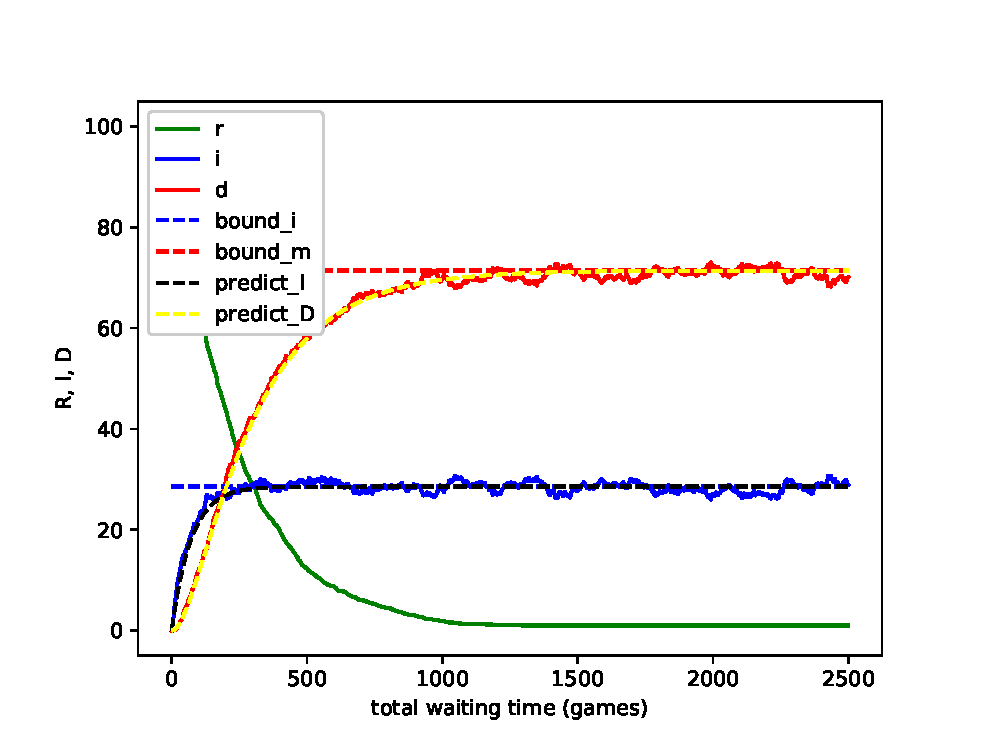
\includegraphics[width=.45\textwidth]{fig/twohop_without_detection.eps}
  \caption{$I(t)$, $D(t)$ and $R(t)$ with time $t$ computed from prediction and simulations
  when $\lambda = 0.004$, $\rho = 0.01$, $N=100$ and $T=2,500$.}
  \label{fig:twohop_predict_wod}
\end{figure}
Fig.~\ref{fig:twohop_predict_wod} shows that the change of the states
in the experiments conforms to the solved solutions (\ref{eq:IDR_wo_solu}).
Here $D(t)$, $I(t)$ and $R(t)$ are the mean values
at the specific time $t$ of $20$ simulations.
We can see from the figure that the $R,I,D$ with
The change of the states
in the experiments conforms to
the solved solutions.

[*** add $R(t)$ ***]
[*** add J P p ***]

\subsection{Efficacy of the approximate method}
\begin{figure}
  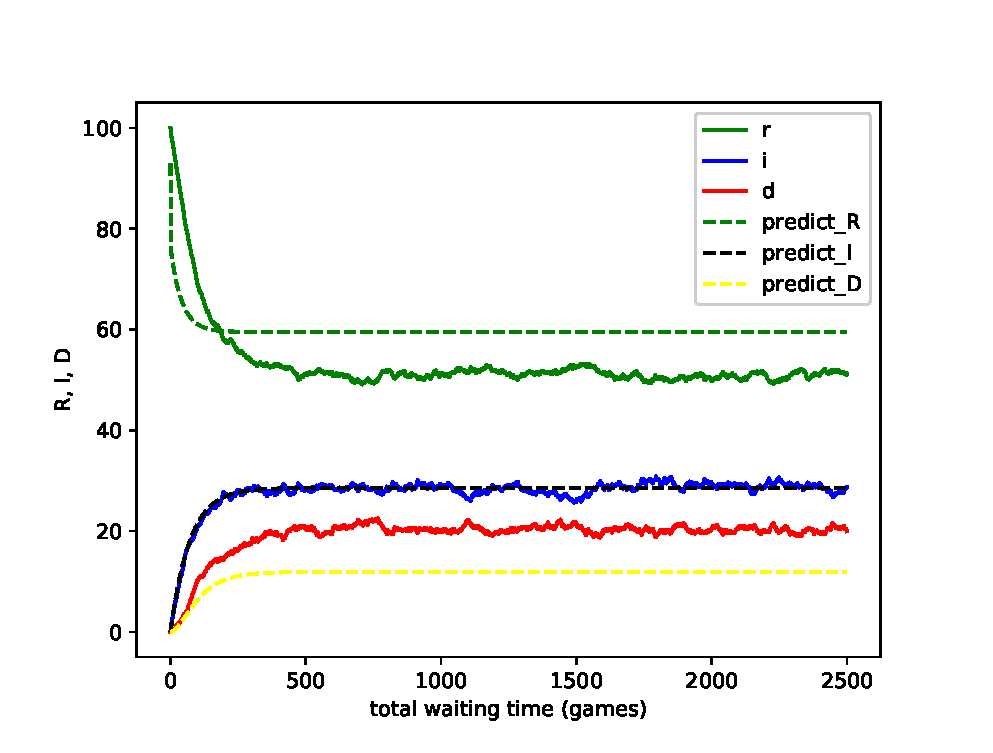
\includegraphics[width=.45\textwidth]{fig/twohop_with_fully_detection.eps}
  \caption{$I(t)$, $D(t)$ and $R(t)$ with time computed from prediction and simulations when $\lambda = 0.004$, $\rho = 0.011$, $N=100$,
  $T_{m} = 1$ and $T=2,500$.}
  \label{fig:twohop_predict_full_d}
\end{figure}
Fig.~\ref{fig:twohop_predict_full_d} shows (\ref{eq:IDR_full}).

\subsection{Optimal solution of selfish detection}
\begin{figure}
  \centering
  {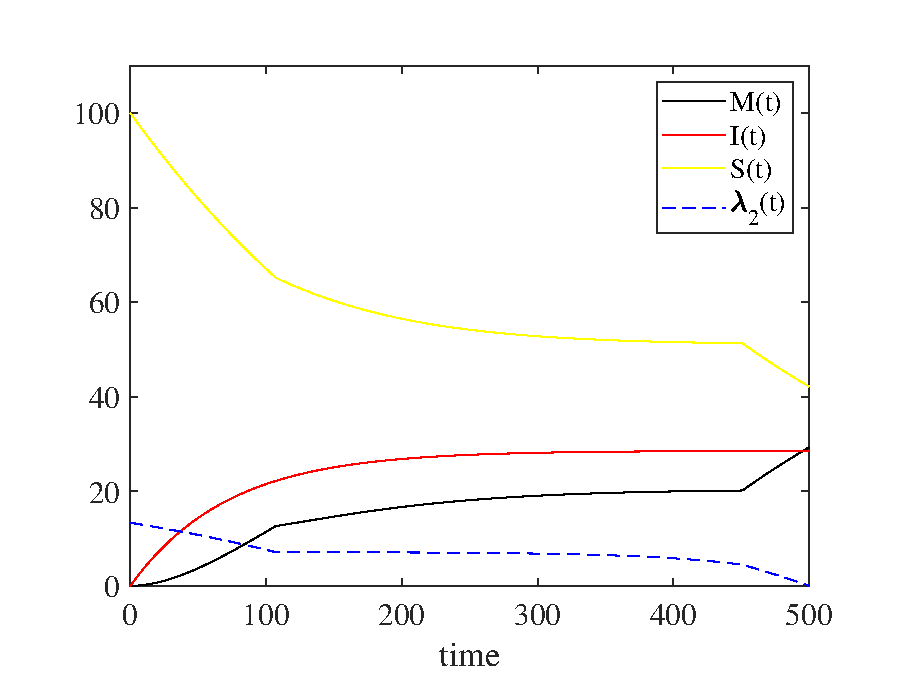
\includegraphics[width=0.47\textwidth]{fig/state.eps}}
     \caption{State variable of analysis with time.}
     \label{fig:pe_opt_state_time}
\end{figure}
\begin{figure}
  \centering
  {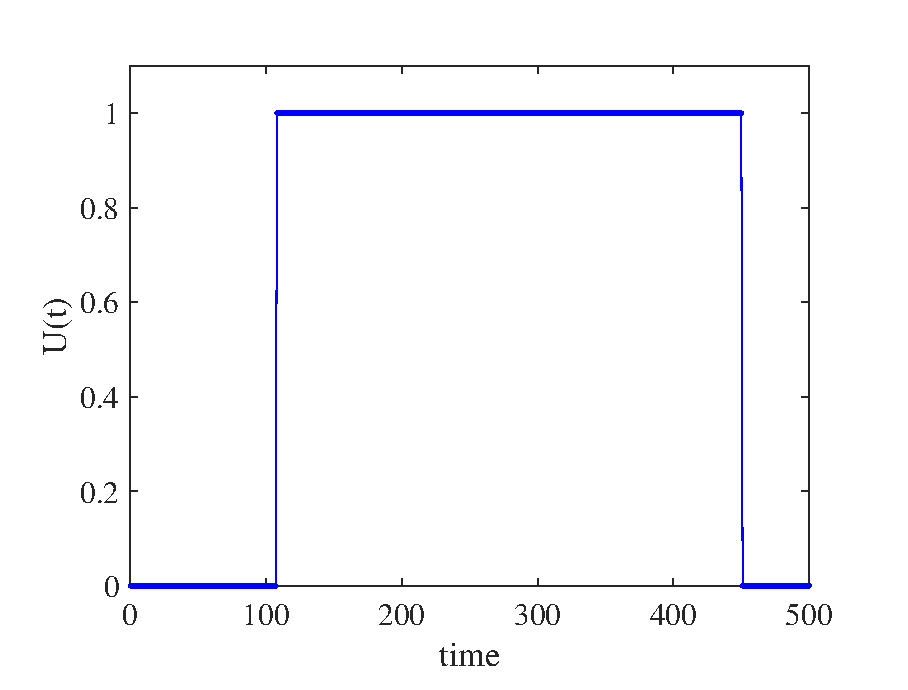
\includegraphics[width=0.47\textwidth]{fig/Ut.eps}}
     \caption{Control variable of analysis with time.}
     \label{fig:pe_opt_control_Ut}
\end{figure}
\begin{figure}
  \centering
  {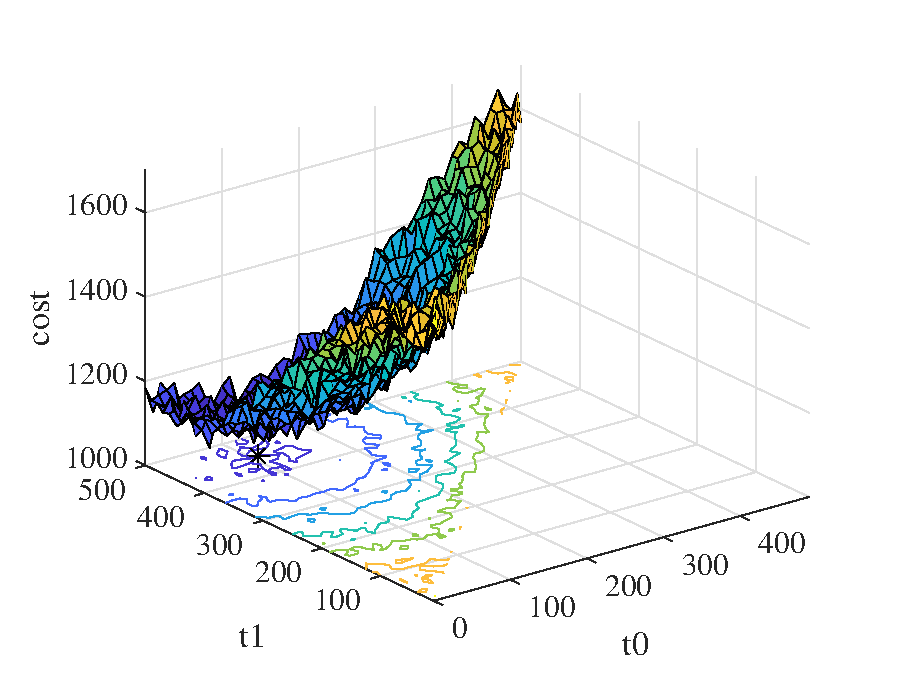
\includegraphics[width=0.47\textwidth]{fig/cost_all_t0t1.eps}}
     \caption{Different choices of $t0$ and $t1$.}
     \label{fig:pe_diff_choices}
\end{figure}

\section{Conclusion}
\label{sec:conclude}


\bibliographystyle{IEEEtran}
\bibliography{reference}

\end{document}
